\documentclass{HZNUMCM}
\usepackage{graphicx}
\usepackage{hyperref}
\usepackage{subcaption}
\usepackage{float}
\definecolor{customcolor}{HTML}{429938}

\setControlNumber{2511940}
\setContestType{MCM}
\setProblemLetter{E}
\setPaperTitle{Our Article}

%summary
\setSummary{ sumary sumary sumary sumary sumary sumary sumary sumary sumary sumary sumary sumary sumary sumary sumary sumary sumary sumary sumary sumary sumary sumary sumary sumary sumary sumary sumary sumary sumary sumary sumary sumary sumary sumary sumary sumary sumary sumary sumary sumary sumary sumary sumary sumary sumary sumary sumary sumary sumary sumary sumary sumary sumary sumary sumary sumary sumary sumary sumary sumary sumary sumary sumary sumary sumary sumary sumary sumary sumary sumary sumary sumary sumary sumary sumary sumary sumary sumary sumary sumary sumary sumary sumary sumary sumary sumary sumary sumary sumary sumary sumary sumary sumary sumary sumary sumary sumary sumary sumary sumary sumary sumary sumary sumary sumary sumary sumary sumary sumary sumary sumary sumary sumary sumary sumary sumary sumary sumary sumary sumary sumary sumary sumary sumary sumary sumary sumary sumary sumary sumary sumary sumary sumary sumary sumary sumary sumary sumary sumary sumary sumary sumary sumary sumary sumary sumary sumary sumary sumary sumary sumary sumary sumary sumary sumary sumary sumary sumary sumary sumary sumary sumary sumary sumary sumary sumary sumary sumary sumary sumary sumary sumary sumary sumary sumary sumary sumary sumary sumary sumary sumary sumary sumary sumary sumary sumary sumary sumary sumary sumary sumary sumary sumary sumary sumary sumary sumary sumary sumary sumary sumary sumary sumary sumary sumary sumary sumary sumary sumary sumary sumary sumary sumary sumary sumary sumary sumary sumary sumary sumary sumary sumary sumary sumary sumary sumary sumary sumary sumary sumary sumary sumary sumary sumary sumary sumary sumary sumary sumary sumary sumary sumary sumary sumary sumary sumary sumary sumary sumary sumary sumary sumary sumary sumary sumary sumary sumary sumary sumary sumary sumary sumary sumary sumary sumary sumary sumary sumary sumary sumary sumary sumary sumary sumary sumary sumary sumary sumary sumary sumary sumary sumary sumary sumary sumary sumary sumary sumary sumary sumary sumary sumary sumary sumary sumary sumary sumary sumary sumary sumary sumary sumary sumary sumary sumary sumary sumary sumary sumary sumary sumary sumary sumary sumary sumary sumary sumary sumary sumary}

%begin
\begin{document}
\showSummarySheet
\showContents

  \section{Introduction}
    \subsection{Background}
      \begin{figure}[ht]
      \centering
        \begin{minipage}[b]{0.45\linewidth}
            \centering
            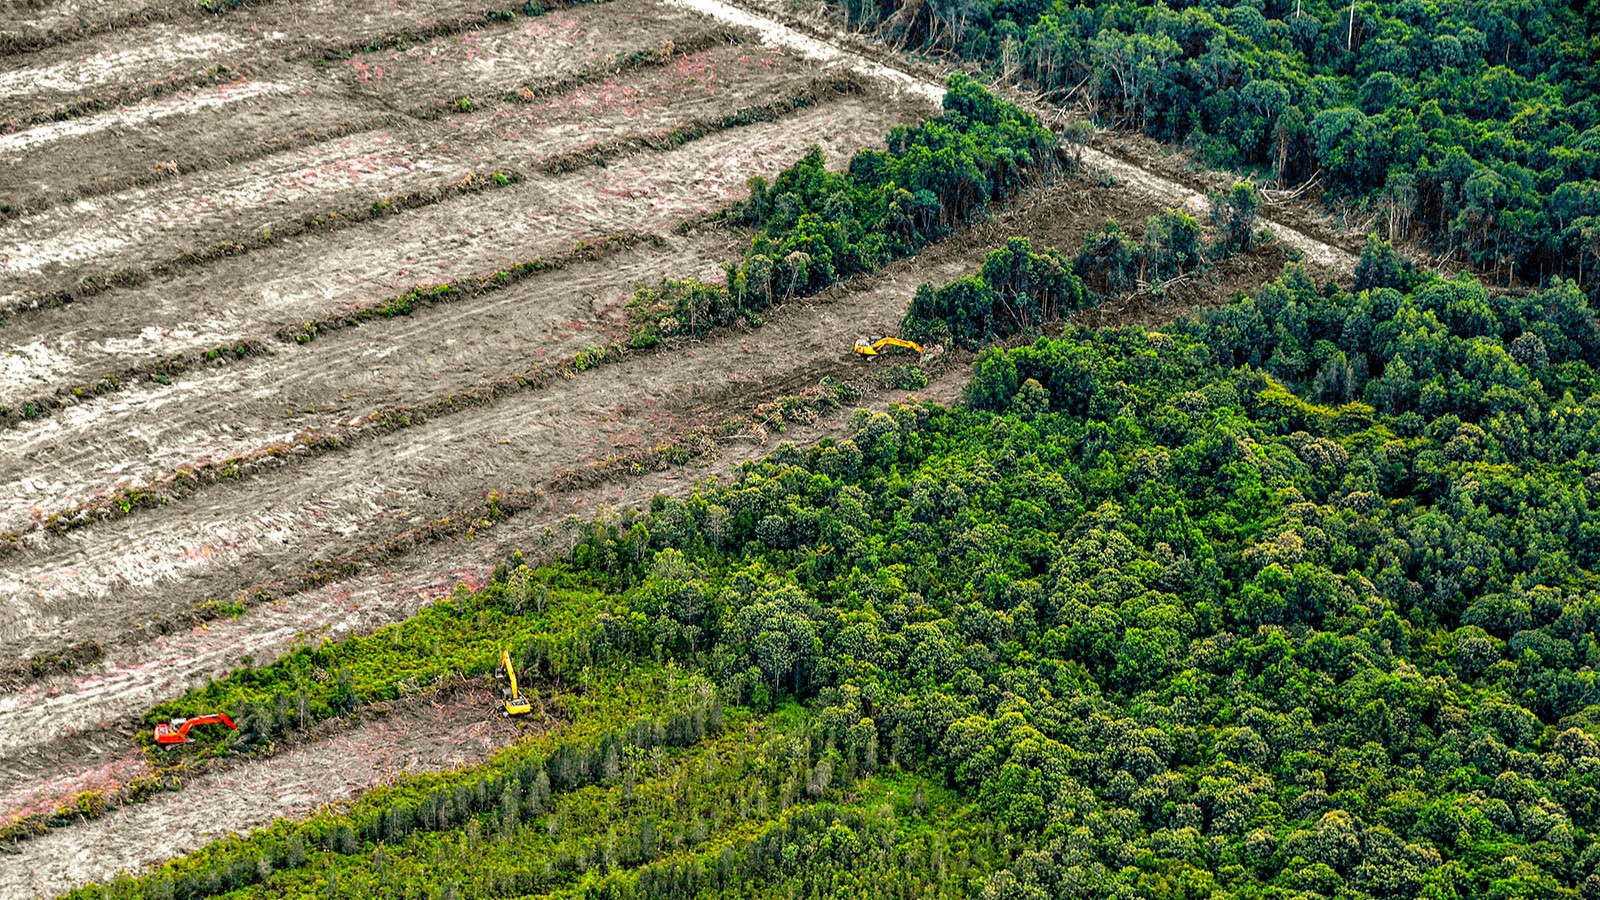
\includegraphics[height=4cm, keepaspectratio]{images/deforestation1.jpg} % 替换为你的第一张图片路径
            \caption{Deforestation for Farming}
            \label{fig:deforestation1}
        \end{minipage}
      \hspace{0.05\linewidth}
        \begin{minipage}[b]{0.45\linewidth}
            \centering
            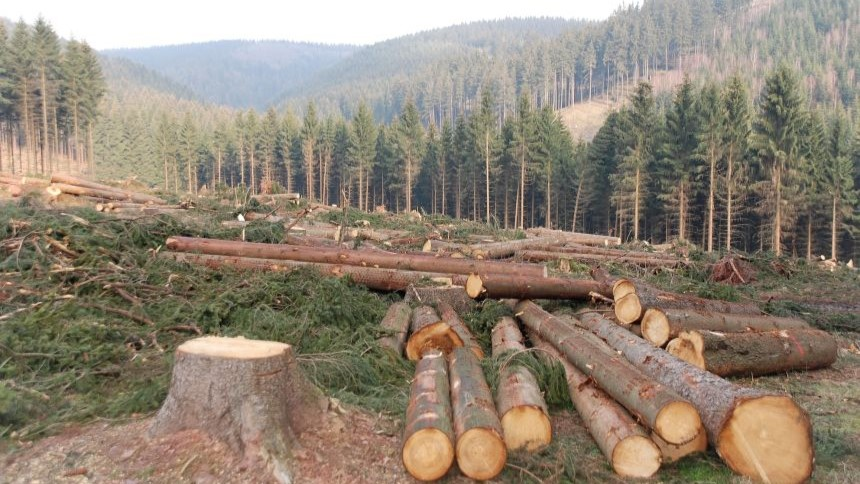
\includegraphics[height=4cm, keepaspectratio]{images/deforestation2.jpg} % 替换为你的第二张图片路径
            \caption{Deforested Forest}
            \label{fig:deforestation2}
        \end{minipage}
      \end{figure}
    \subsection{Problem Analysis}
    \subsection{Our Work}
    \begin{itemize}
      \item 1
      \item 2
      \item 3
    \end{itemize}

  \section{Assumptions and Notations}
    \subsection{Assumptions and Explanations}
      \begin{itemize}
        \item \textbf{Accurate Data Assumption}: The model assumes that the data used are accurate.\\
        \textbf{Explanation}: The data used in the model are sourced from official databases, and we believe the data to be accurate and reliable.
        
        \item \textbf{Geographic Applicability Assumption}: The model assumes that the applicable region is Southeast Asia,
         where two crops of rice are planted each year in the farmland.\\
        \textbf{Explanation}: The climate of Southeast Asia is rather simple, 
        with only two seasons-rainy and dry. Additionally, as is shown in \figurename~\ref{fig:Temperature},
        the temperature variation within a year is minimal,which has a trivial effect on the ecosystem.
        Consequently,temperature can be considered as a constant.
        Due to such weather pattern,it aligns with the planting patterns commonly observed in Southeast Asia to plant two crops of rice each year,
         and the simplicity of crop types makes the model easier to establish.
        
        \begin{figure}[H]
          \centering
          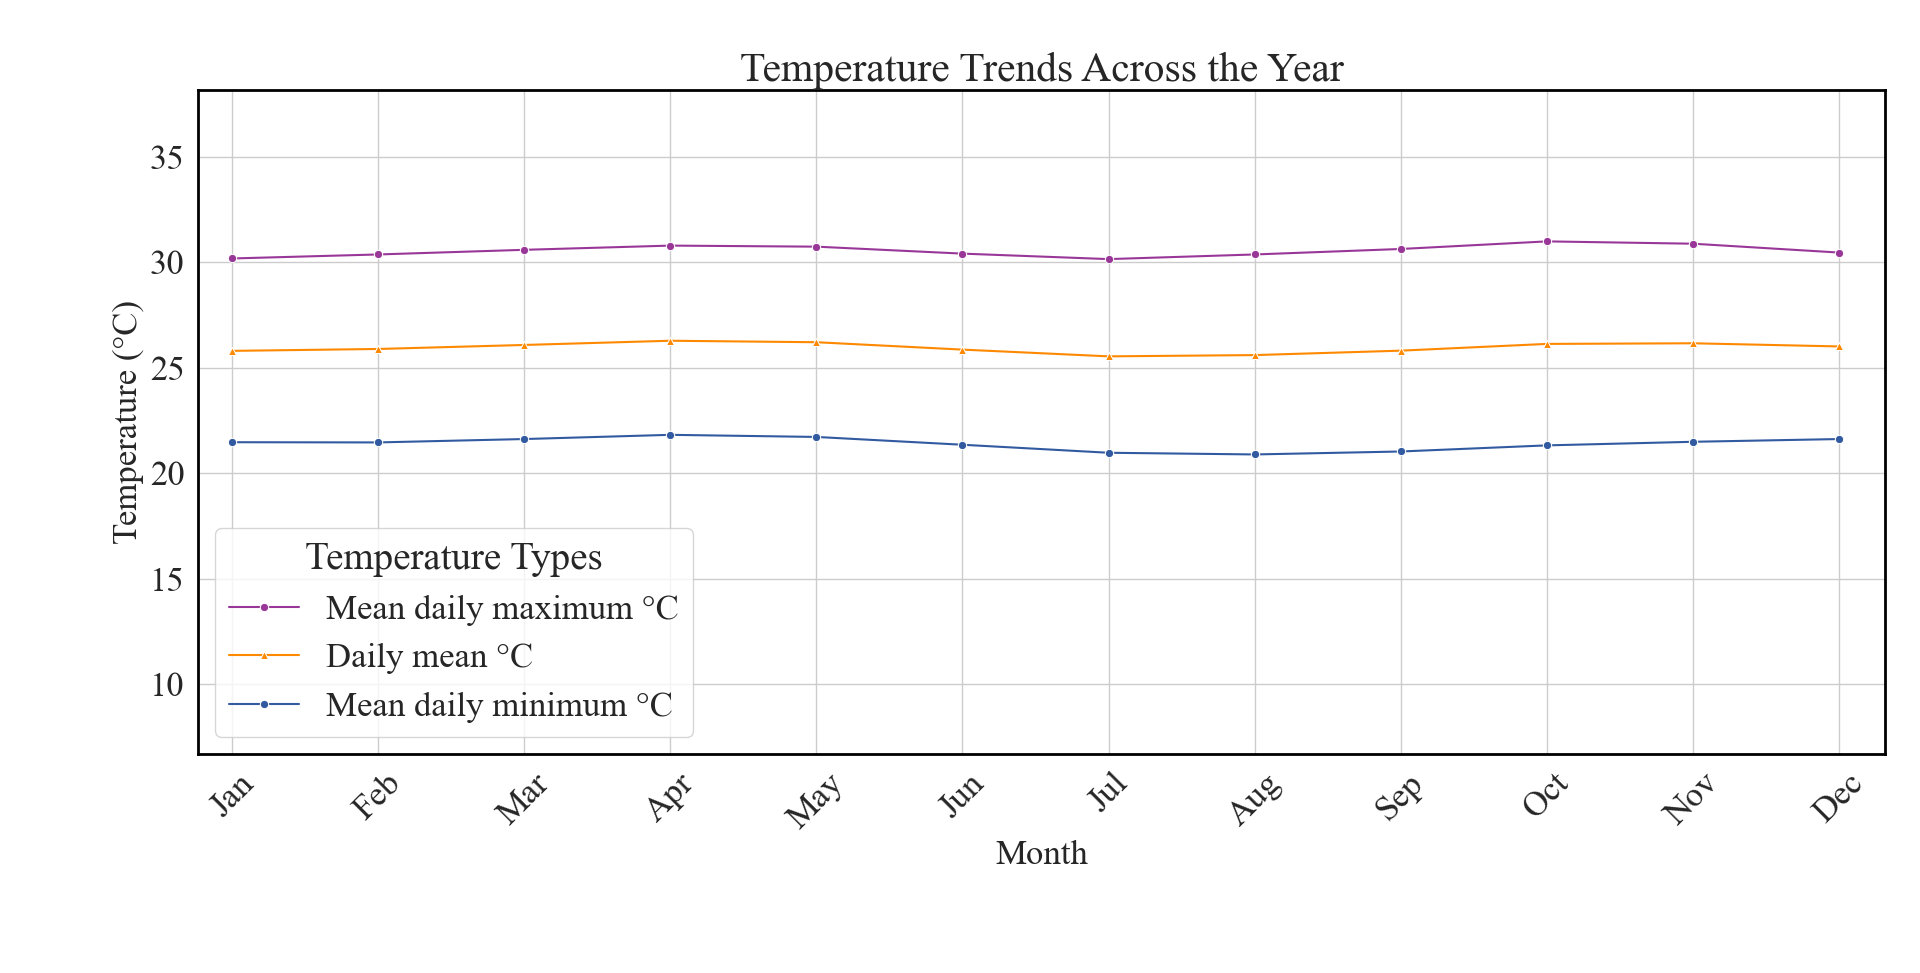
\includegraphics[width=\linewidth]{images/AverTemper.png}
          \caption{Mean Temperature from 1991 to 2020 in Southeast Asia}
          \label{fig:Temperature}
        \end{figure}

        \item \textbf{Stable Trait Assumption}: The model assumes that the traits of all organisms remain stable..\\
        \textbf{Explanation}:Since the time span considered in the model is much shorter than the time required for evolutionary changes or mutations to occur,
         the traits of organisms are assumed to remain stable. This assumption also helps simplify the model.
        
        \item \textbf{Stable Lighting Conditions Assumption}: The model assumes that the region under study experiences stable lighting conditions throughout the four seasons.\\
        \textbf{Explanation}: Since the model focuses on tropical regions, the variation in daylight duration across different months within a year is minimal,
         thus the lighting conditions are treated as constant in the model.
        
        \item \textbf{Stable Growth Environment Assumption}: The model assumes that no natural disasters,
         which could significantly impact the agricultural ecosystem, will occur during the time frame considered.\\
        \textbf{Explanation}: Natural disasters are considered low-probability events in agricultural activities.
         To ensure the generalizability of the model, natural disasters should not be considered.
      \end{itemize}

        \subsection{Notations}
      % table
      \begin{table}[H]
        \centering
        % \caption{An example of a three-line table.}
        \begin{tabular}{cc}
          \toprule
          \rowcolor{customcolor!40} % 设置背景颜色
          Symbols & Description\\
          \midrule
          $\mathbf{X}$ & Vector $[N_{wd},N_{crp},N_{pst},N_{ins},...,C_{hc},C_{pc}]^T$ to describe the system,etc. \\
          $wd$ & Subscription for weeds \\
          $crp$ & Subscription for crops \\
          $pst$ & Subscription for pest(who consumes crops) \\
          $ins$ & Subscription for other insects(who consume weeds) \\
          $bd$ & Subscription for small birds(herbivorous) \\
          $Bd$ & Subscription for huge birds(carnivorous) \\
          $bt$ & Subscription for bats \\
          $snk$ & Subscription for snake \\
          $frg$ & Subscription for frog \\
          $HC$ & Subscription for herbicide \\
          $PC$ & Subscription for pesticide \\
          $C_i$ & Concentration of certain chemical \\
          $N_i$ & Numbers of certain species \\
          $W_i$ & Biomass of certain species \\
          $w_i$ & Mass of individuals \\
          $r_i$ & Natural growth gate of certain species\\
          $K_i$ & Carrying capacity of certain species\\
          $\alpha$ & The effect of chemical concentration on growth rate\\
          $\beta$ & Interspecific competition factor\\
          $\gamma$ & Activity of decomposer\\
          
          \bottomrule
        \end{tabular}
        \label{tab:example}
      \end{table}

  \section{Models}
    %     % figure
    % \begin{figure}[ht]
    %   \centering
    %   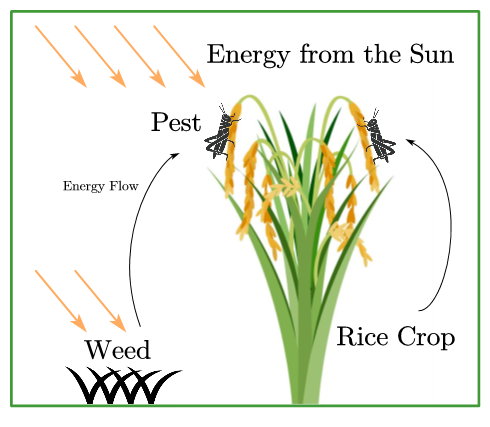
\includegraphics[width=0.5\linewidth]{images/energy_flow.png} % 替换为你的第一张图片路径
    %   \caption{Energy Flow}
    %   \label{fig:EnergyFlow}
    % \end{figure}
    \subsection{NGLG(Natrual Growth Leslie-Gower) Model}
      \subsubsection{Leslie-Gower Model}
        Ecosystem components are complex and interdependent. 
        In the simplest case, when climate, soil, and other conditions are favorable, only biological factors shuold be considered. 
        If the population sizes of producers, primary consumers, and secondary consumers are used to describe the entire system, 
        the Leslie-Gower Model, as described by \cite{GUO20142850}, can be applied.
        \begin{equation}
          \left\{ \begin{array}{c}
            \frac{\mathrm{d}N_1\left( T \right)}{\mathrm{d}T}=r_1N_1\left( T \right) \left( 1-\frac{N_1\left( T \right)}{K_1} \right) -\alpha _1N_2\left( T \right) ,\\
            \frac{\mathrm{d}N_2\left( T \right)}{\mathrm{d}T}=r_2N_2\left( T \right) \left( 1-\frac{N_2\left( T \right)}{c_1X\left( T-\tau _1 \right)} \right) -\alpha _2Z\left( T \right) ,\\
            \frac{\mathrm{d}N_3\left( T \right)}{\mathrm{d}T}=r_3N_3\left( T \right) \left( 1-\frac{N_3\left( T \right)}{c_2N_2\left( T-\tau _2 \right)} \right)\\
          \end{array} \right. 
        \end{equation}
        In the equations,$N_1,N_2,N_3$ represents producers, primary consumers, and secondary consumers, respectively; 
        $c_1>0$ and $c_2>0$ are the measure of food quality measure that prey provides for conversion into the births of consumer and predator; 
        the positive parameters $a_1$ and $a_2$ are the predation rate of consumer and predator; 
        two delays $\tau_1, \tau_2>0$ are introduced for digestion periods corresponding to consumer-eat-resource and predator-eat-consumer, 
        which are called the resource digestion delay (RDD) and consumer digestion delay (CDD), respectively.
        It is a schematic diagram of this model.
      \subsubsection{NGLG Model}
        
  \section{Application of the Models}

  \section{Sensitivity Analysis}

  \section{Evaluation of the Model}
    \subsection{Strengths}
    \subsection{Weaknesses}

  \section{Conclusion}

  % % figure
  % \begin{figure}[ht]
  %   \centering
  %   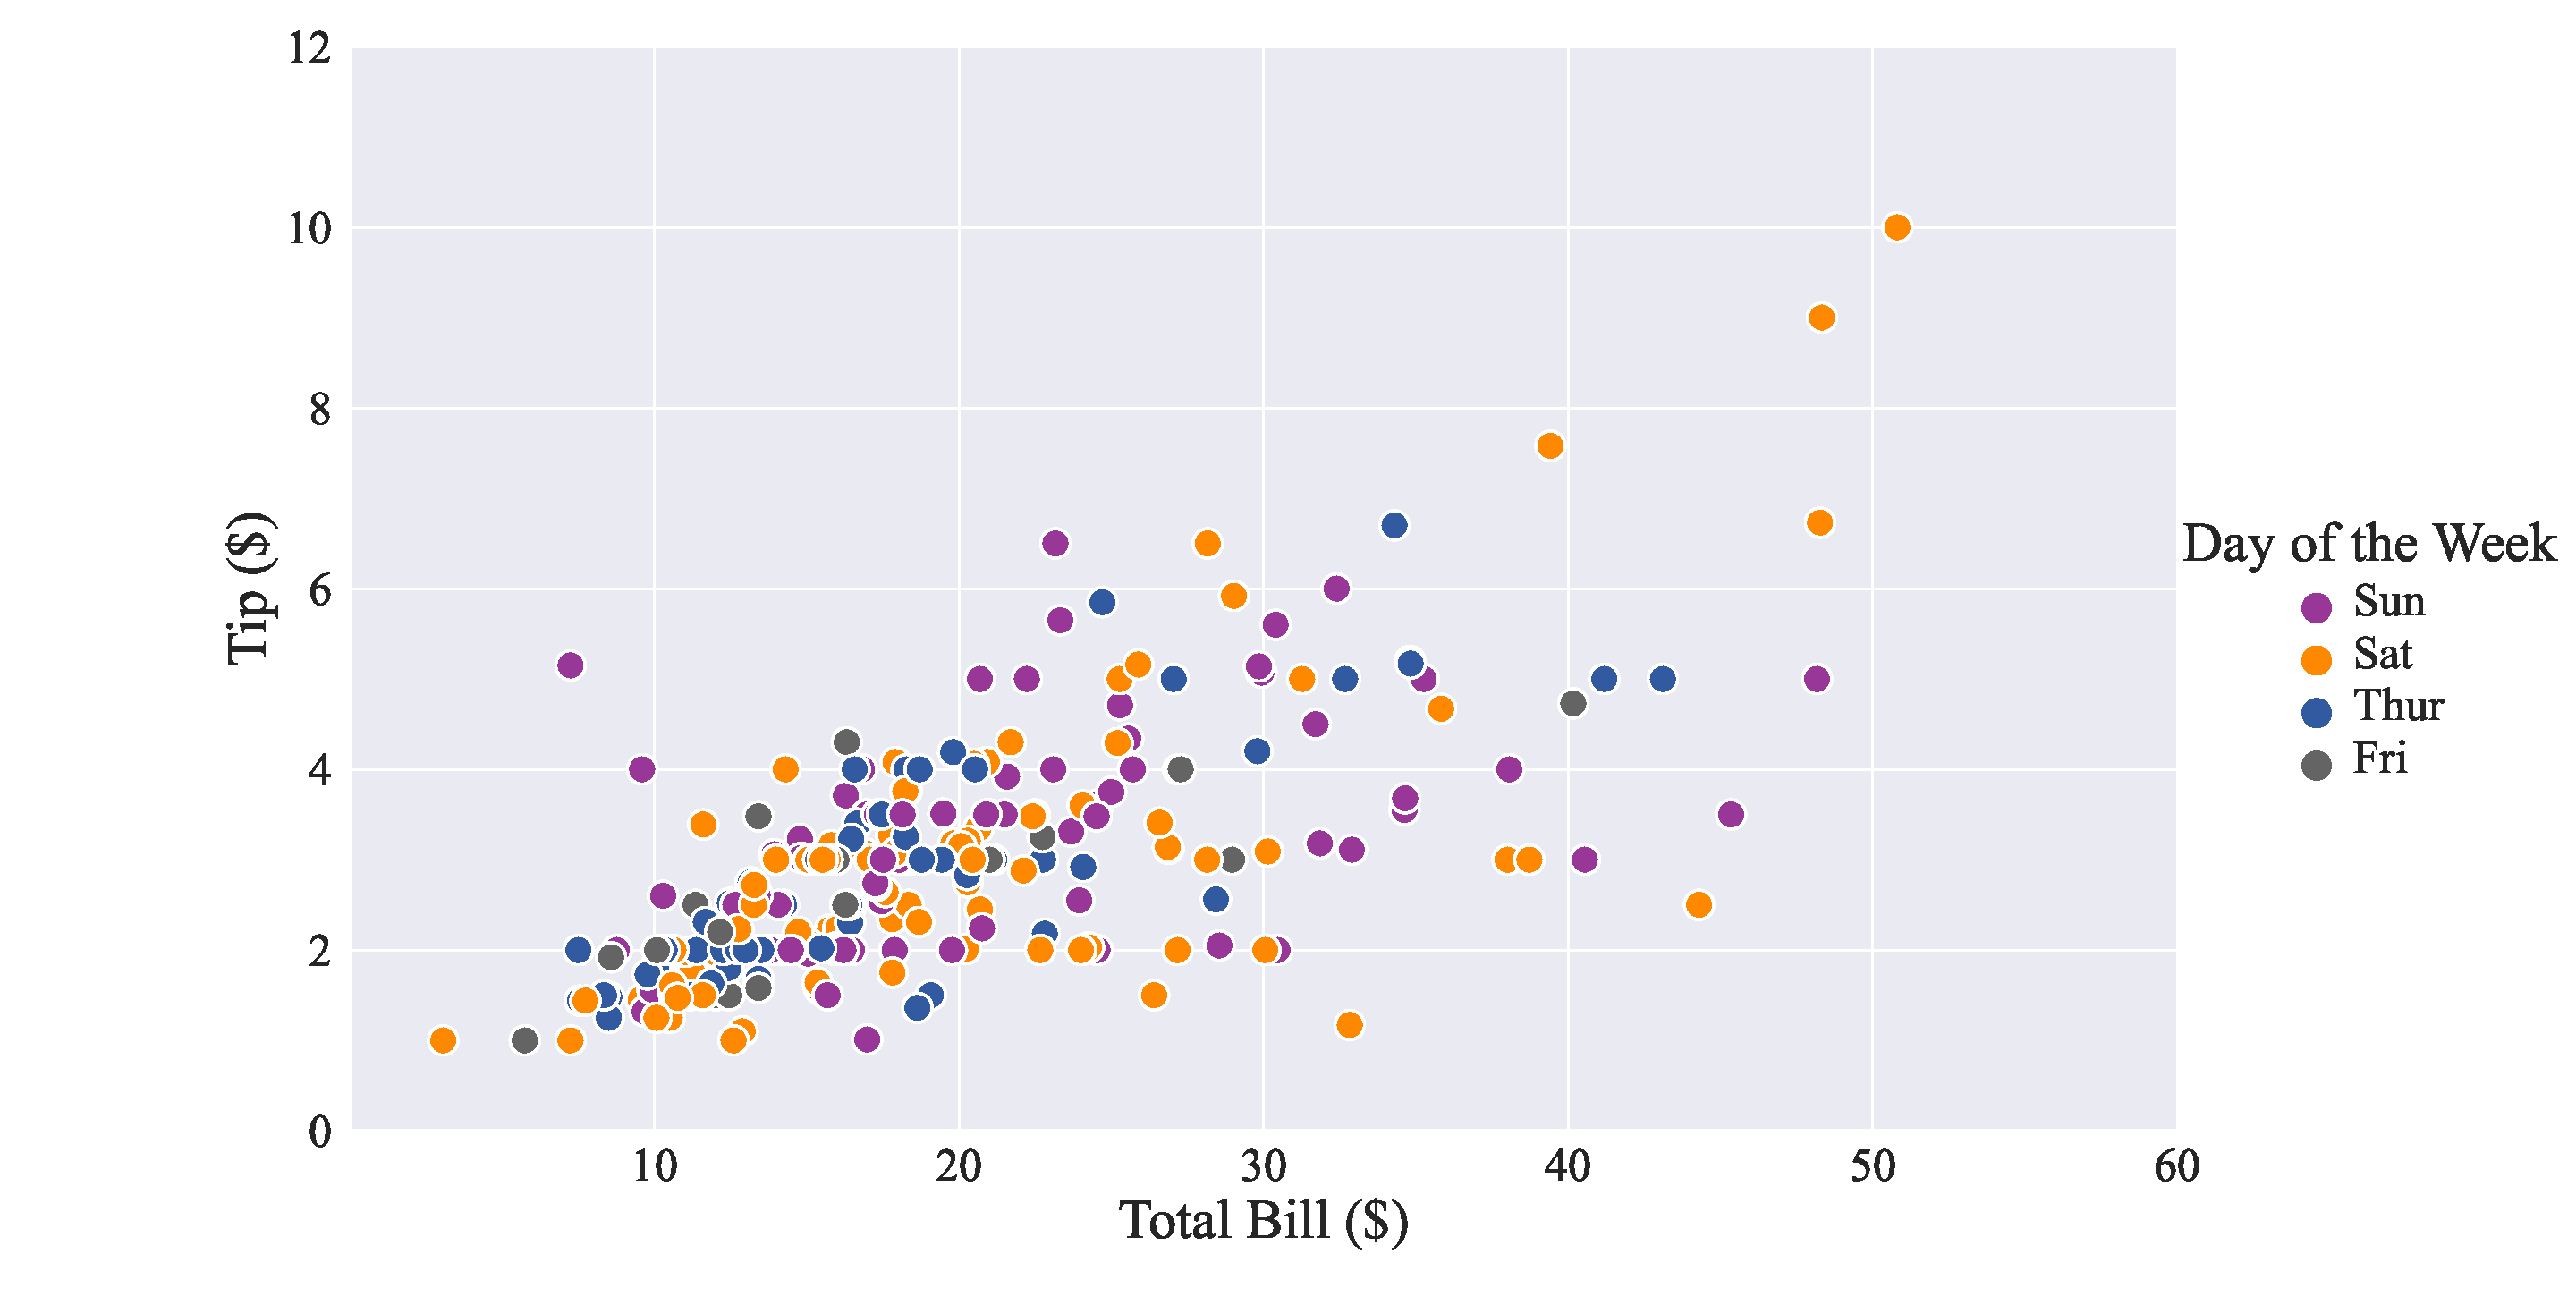
\includegraphics[width=\linewidth]{images/scatter.pdf} % 替换为你的第一张图片路径
  %   \caption{the scatter}
  %   \label{fig:image1}
  % \end{figure}

  % \begin{figure}[ht]
  %     \centering
  %     \begin{minipage}[b]{0.45\linewidth}
  %         \centering
  %         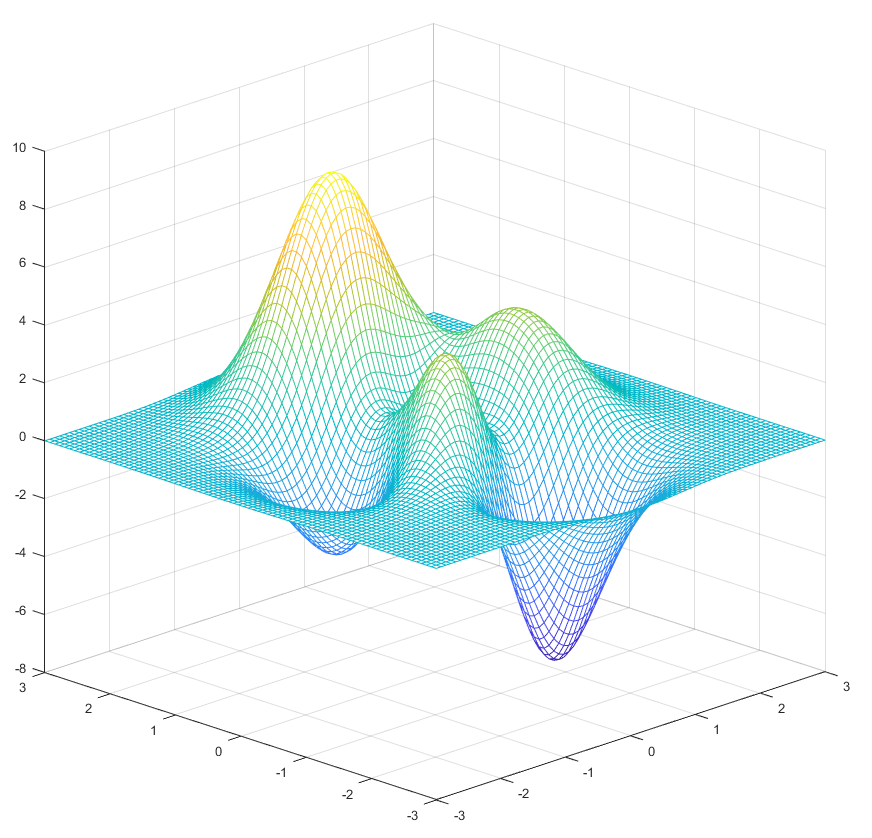
\includegraphics[height=5cm, keepaspectratio]{images/peaks.png} % 替换为你的第一张图片路径
  %         \caption{First Image}
  %         \label{fig:image2}
  %     \end{minipage}
  %     \hspace{0.05\linewidth}
  %     \begin{minipage}[b]{0.45\linewidth}
  %         \centering
  %         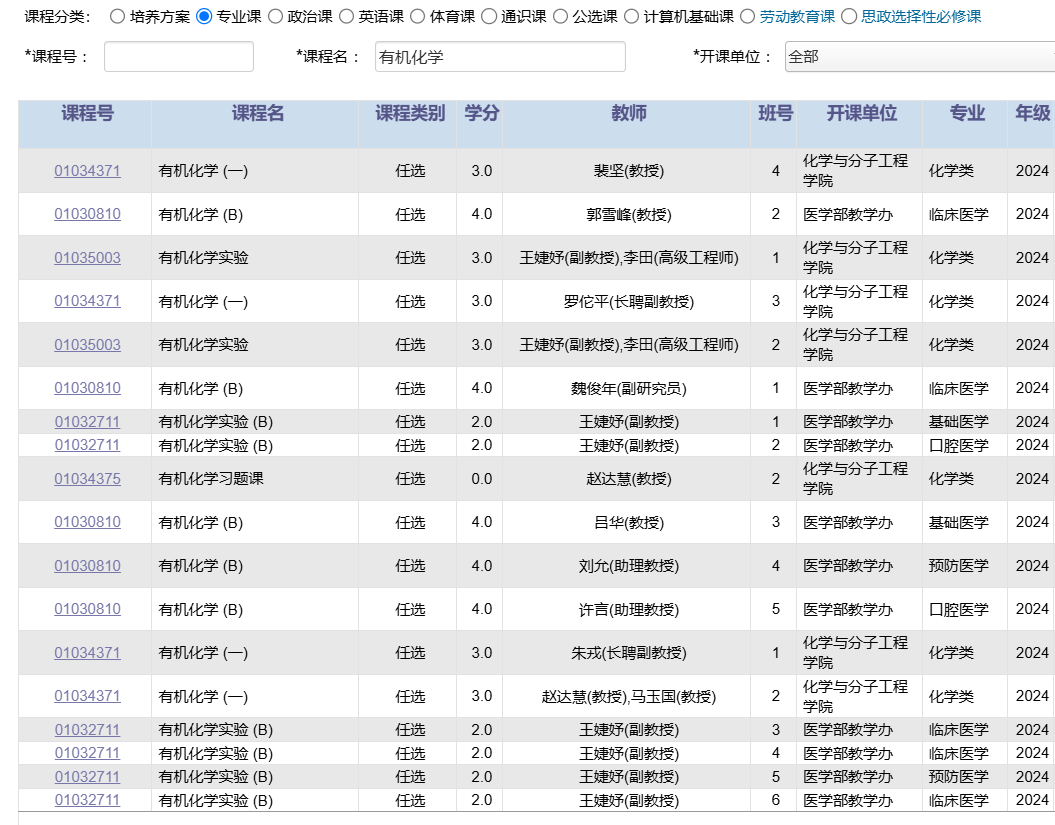
\includegraphics[height=5cm, keepaspectratio]{images/courses.png} % 替换为你的第二张图片路径
  %         \caption{Second Image}
  %         \label{fig:image3}
  %     \end{minipage}
  % \end{figure}

  %%citation
  % as \figurename~\ref{fig:image1} shows,this is a picture.
  % ...\cite{example1}
  % 123123123\cite{rosenow1983drought}

  % % table
  % \begin{table}[h]
  %   \centering
  %   \caption{An example of a three-line table.}
  %   \begin{tabular}{lccc}
  %     \toprule
  %     \rowcolor{customcolor!50} % 设置背景颜色
  %     Column 1 & Column 2 & Column 3 & Column 4 \\
  %     \midrule
  %     Data 1 & Data 2 & Data 3 & Data 4 \\
  %     Data 4 & Data 5 & Data 6 & Data 8 \\
  %     \bottomrule
  %   \end{tabular}
  %   \label{tab:example}
  % \end{table}

  \addcontentsline{toc}{section}{References}
  \bibliographystyle{unsrt}%{brief}%{alpha}%{unsrt}
  \bibliography{article_file}

\end{document}